




\documentclass[12pt]{article}
\usepackage{color}
\usepackage{tabularx}
\usepackage{multirow}
\usepackage{csvsimple}
\usepackage{mhchem}
\usepackage{graphicx}
\usepackage{subcaption}
\usepackage{mwe}
\usepackage{float}
\usepackage{placeins}
\usepackage{amsfonts}
\usepackage{booktabs}
\usepackage{siunitx}
\usepackage{array}
\usepackage{pdfpages}
\usepackage{pdflscape}





\title{Modelling the Transition to a Low-Carbon Electricity Supply}
\author{Alexander Kell \\ {A.Kell2@newcastle.ac.uk}}

\date{\today}


\begin{document}

\maketitle

\clearpage

\section{Background and Research Question}

%\subsection{Background and research question}


Due to the threat of climate change, a transition from a fossil-fuel based system to one based on zero-carbon is required. However, this is not as simple as shutting down all fossil-fuel based power plants and replacing them with renewable energy; careful decisions need to be made to reduce economic impact and lapses in electricity supply. Decision makers, therefore, need a way of assessing the consequences of decisions in different possible scenarios. 

Due to a deliberate move away from centralised planning, and to the liberalisation of electricity markets in many western democracies, heterogenous actors with bounded rationality and imperfect information should be focused on to increase understanding \cite{Kraan2018}. Traditional optimisation models use a typical cost-optimal allocation, for a range of climate objectives. However, historically, this is not necessarily how emission reductions occur, due to various factors such as the inertia of different sectors within the energy system, governance and national political priorities  \cite{PyeS.PriceJ.CroninJ.ButnarI.andWelsby2019}.

I propose a method of modelling these heterogenous actors in electricity markets and explore potential pathways to transition to a low-carbon economy. For this goal, I have created a new open-source agent-based model named ElecSim. ElecSim is a stochastic electricity market simulation tool which enables practitioners to alter scenarios and assess the outcomes of possible interventions in an electricity market, enabling one to observe the decision of individual companies as opposed to a centralised planner.

I propose the use of artificial intelligence and optimisation techniques to gain a more realistic representation of an electricity market, and better aid policy makers and electricity market players. Specifically, this will involve the use of reinforcement learning techniques such as Deep Deterministic Policy Gradients (DDPGs)\cite{Hunt2016}, or Deep Q Networks \cite{Mnih2013}. These algorithms will be used to learn optimal bidding and investment strategies.


\paragraph{Literature Review}

Live experimentation of an electricity market is not practical. The time scales are long and there is a significant risk that changes can have detrimental impacts. This can often lead to minor tweaks being made \cite{Forshaw2016}. A solution to this is simulation, where simulation is the substitution of a physical process with a computer model.

A number of different simulations and computer models have been used to aid policy makers and energy market developers in  coming to informed conclusions. Energy models can typically be classified as top-down macro-economic models or bottom-up techno-economic models \cite{Bohringer1998}. To explicitly model types of technology such as the intermittency of renewables we have focused on bottom-up techno-economic models.

It is possible to further categorise bottom-up models into optimisation and simulation models. Optimisation energy models minimise costs or maximise welfare, defined as the material and physical well-being of people, from the perspective of a central planner ~\cite{Keles2017}. Examples of optimisation models are MARKAL/TIMES~\cite{Fishbone1981} and MESSAGE~\cite{Schrattenholzer1981}. 

However, electricity market liberalisation in many western democracies has changed the framework conditions. Centralised, monopolistic, decision making entities have given way to multiple heterogeneous agents acting for their own best interest~\cite{Most2010}. Policy options must therefore be used to encourage changes to attain a desired outcome. It is proposed that these complex agents are modelled using ABMs due to their non-deterministic nature. 



\begin{table}[]
	%	\begin{tabular}{|l|c|c|c|c|c|}
	\begin{tabular}{m{2.5cm}m{1.2cm}m{1.5cm}m{2cm}m{2cm}m{2cm}} \toprule
		\multicolumn{1}{c}{\textbf{Tool name}} & \textbf{Open Source} & \textbf{Long-Term Investment} & \textbf{Market} & \textbf{Stochastic Inputs} & \textbf{Country Generalisability} \\ \midrule
		SEPIA \cite{Harp2000}  & \checkmark           & $\times$                             & \checkmark      & Demand                     & \checkmark                        \\ 
		EMCAS ~\cite{Conzelmann}   & $\times$                    & \checkmark                    & \checkmark      & Outages                    & \checkmark                        \\ 
		NEMSIM ~\cite{Batten2006}  & ?              & \checkmark                    & \checkmark      & $\times$                          & $\times$                                 \\ 
		AMES  ~\cite{Sun2007} & \checkmark           & $\times$                             & Day-ahead       & $\times$                          & $\times$                                 \\ 
		GAPEX  ~\cite{Cincotti2013} & ?              & $\times$                             & Day-ahead       & $\times$                          & \checkmark                        \\ 
		PowerACE \cite{Rothengatter2007} & $\times$                    & \checkmark                    & \checkmark      & Outages Demand             & \checkmark                        \\ 

		EMLab ~\cite{Chappin2017}  & \checkmark           & \checkmark                    & Futures         & $\times$                          & \checkmark                        \\ 
		MACSEM  ~\cite{Praca2003}  & ?              & $\times$                             & \checkmark      & $\times$                          & \checkmark                        \\ 
		ElecSIM                                  & \checkmark           & \checkmark                    & Futures         & \checkmark                 & \checkmark                        \\ \hline
	\end{tabular}
	\caption{Features of electricity market ABM tools.}
	\label{table:tool_comparison}
\end{table}



A number of dedicated tools have been created for this regard, however by referring to Table \ref{table:tool_comparison} it can be seen that these do not suit the needs of an open source, long-term market model.







%\subsection{Background and Research Question}



%
%\begin{itemize}
%  \item Introduction to problem of climate change and requirement for decarbonization.
%  \item Requirement of shift in heating, transport, and industry to electricity.
%  \item Inability to use traditional machine learning and statistical tools to project into future due to rapid disruption.
%  \item Use of long-term agent-based model to simulate into the future (eg. 2050) allowing policy makers and energy market players to assess effect of decisions made.
%  \item Agent-based models can be used to model the impact of heterogenous investors
%  \item Enable policy makers to assess the impact of market power and collusion
%  \item Ability to use reinforcement learning to give agents intelligence
%\end{itemize}
%
%\subsection{Literature Review}
%
%\begin{itemize}
%  \item  Literature review on state-of-the-art models and applications
%  \item Agent-based model tools
%  \begin{enumerate}
%  	\item Absence of open-source tool with stochasticity (table).
%  \end{enumerate}
%
%  \item Optimisation tools
%\end{itemize}


%\subsection{Work Completed}
%
%\begin{itemize}
%  \item Short-term load forecasting
%  \item Completion of agent-based model at yearly granularity
%  \item Results of yearly granularity of agent-based model
%  \item Use of Northern Ireland scenario for optimisation of carbon tax using reinforcement learning (preliminary results)
%\end{itemize}





\clearpage

\clearpage

\section{Research Outputs}

\paragraph{A. Kell, A. S. Mcgough, and M. Forshaw, ``Segmenting Residential Smart Meter Data for Short-Term Load Forecasting.'' e-Energy Conf., pp. 91--96, 2018. \cite{Kell2018}
}


In this work, we compared machine learning techniques at their ability to predict electricity demand 30 minutes ahead. For this, we utilised smart meter data data obtained from the Irish Social Science Data Archive \cite{cer_2012}.

We used K-means clustering \cite{Forgy65} to cluster similar households, and predicted the scaled aggregate of these clusters. A variety of different forecasting techniques were evaluated such as Random Forests \cite{TinKamHo}, Long Short-Term Memory Neural Networks \cite{lstm}, Artificial Neural Networks \cite{book:984557} and Support Vector Regression \cite{Drucker1997}. We found that random forests performed best for our scenario.


\paragraph{A. Kell, M. Forshaw, and A. S. McGough,  ``ElecSim: Stochastic Open-Source Agent-Based Model to Inform Policy for Long-Term Electricity Planning.''  e-Energy Conf., 2019.
}

We have had the aforementioned paper accepted to be published in the e-Energy '19 Electricity Market Engineering Workshop.

In this paper we detail the technical details of ElecSim. We detail scenarios where we reduce electricity demand by 1\% a year. We also vary carbon tax and demonstrate that starting from a low value of \textsterling26 and increasing linearly to \textsterling150, as predicted by the UK government BEIS \cite{Department2016}, leads to a lower uptake of renewables by 2050 than maintaining a carbon tax of \textsterling40.

\paragraph{A. Kell, M. Forshaw, and A. S. McGough, ``Modelling Carbon Tax in the UK Electricity Market using an Agent-Based Model''. e-Energy Conf., 2019.}

We have had the aforementioned paper accepted to be published as a poster. In this work we provide further scenarios by using the ElecSim model and set carbon tax to equal \textsterling10, \textsterling20, and \textsterling70. We found that a carbon of \textsterling10 was insufficient to cause a significant uptake in renewable energy. However, a carbon tax of \textsterling70 lead to an almost 100\% renewable energy supply by 2050.


\paragraph{Internship at Centre for Science and Policy, University of Cambridge}

At this internship I will be working with policy advisers from across the world, and with academics to increase research impact for policy. This will give me an insight into governmental policy, and will help to form the policy issues most related to my PhD, and how to present this to policy makers.

\clearpage

\section{Remaining Work}

Whilst the agent-based model, ElecSim, has been designed and parametrised, it has been designed to cater for a temporal granularity of a yearly time-step. That is, decisions for bidding into an electricity market and investing in power plants happens every year. The goal is to increase the granularity temporally, which will enable the modelling of sudden fluctuations in wind speed and solar irradiance. Collins \textit{et al.} showed that a low temporal resolution results in overestimation of intermittent renewable energy technology, and underestimation in dispatchable energy sources \cite{Collins2017}.

To further increase the validation accuracy of ElecSim, I propose the use of optimisation such as mixed integer linear programming and genetic programming to further parametrise the model. I propose the use of the NSGA-II algorithm, which enables multi-objective optimisation, and approximates the pareto frontier \cite{Valkanas2014}. I propose the minimisation of the difference between real and modelled electricity prices and real and modelled energy mix. Where the energy mix is defined as percentage share of different energy types.

I propose the use of reinforcement learning techniques to control the behaviour of agents. For instance, controlling and optimising the behaviour of investment decisions and bidding strategies. I would also like to model collusion between agents through the means of parameter sharing between agents. This would enable the comparison between scenarios where collusion is present and those where it is not.

Whilst I have completed preliminary work on optimising the carbon price using reinforcement learning techniques using DDPG, I would like to do improve this when I have designed a higher granularity model to improve results.

I propose the modelling of further scenarios using this model and change variables such as cost of technologies, change in demand, uncertainty in fuel prices, differing countries, and changing availability and capacity factors.

Finally, I would like to compare my model to another open source model, OSeMOSYS \cite{Howells2011}. OSeMOSYS is an optimisation based model. I believe that a comparison between agent-based models and optimisation model will help to elucidate the strengths and weaknesses of these models in comparison to one another, and discover the scenarios in which the models are better suited. 

%\begin{enumerate}
%  \item Increase granularity to hourly.
%  \begin{enumerate}
%  \item Selection of best representative days for long-term - Comparison to literature that selects best day for single year.
%  \end{enumerate}
%  \item  Parametrise model using genetic algorithm or other optimisation tool.
%
%  \item Add intelligence to agents using reinforcement learning for:
%  \begin{enumerate}
%      \item Investment decisions.
%      \item Bidding strategy.
%      \item Impact of collusion (variable sharing between two or more agents).
%  \end{enumerate}
%  \item Complete work on carbon tax optimiser
%  \item Comparison of optimisation and agent-based model in different scenarios.
%  \begin{enumerate}
%  \item Same intialisation parameters and project to future (form of cross-validation).
%  \item Collusion.
%  \end{enumerate}
%  \item Further scenarios and results as examples
%  \begin{enumerate}
%  \item Decreasing costs of technology over time
%  \item Different countries
%  \item Improving availability and capacity factors
%  \item Uncertainty in fuel prices
%  \item Changing demand curve shape due to increase in electric vehicles
%\end{enumerate}
%
%\end{enumerate}




\clearpage

\section{Progress against First Year Plan}

\paragraph{Review}

A literature review has been undertaken and a greater understanding of energy market models has been developed. With a distinction between top-down macroeconomic models and bottom-up techno-economic models shown. Also the differences between traditional centralised optimisation models and new simulation techniques developed. I have developed a table which positions my research in relation to the literature. I will further the review to explore the nuances in the binary responses given in the columns "Country Generalisability".

\paragraph{Design of System and Validation}

The fundamental components of the system have been designed. A model of an electricity market with a yearly time-step has been completed with generation company and demand agents, and example scenarios. The model has been calibrated with data from the UK, however designed in such a way that other countries can be used. For instance, by providing an optimisation framework in which individual cost parameters can be estimated from a simple average cost of electricity.

I am currently testing the design of a 30 minute time step. Representative days of weather and load have been selected to reduce overall computation time by testing different techniques such as k-means clustering \cite{Forgy65}, genetic programming, such as the NSGA-II \cite{Valkanas2014} and Fourier resampling \cite{Cooley2006}. 

The model has been validated through the comparison of actual electricity prices with modelled electricity prices, with a normalised root mean square error of \textsterling4.41/MWh. Improving on the non-stochastic case by 52.5\%. The model has also been validated through the means of observation of a process. Specifically, an increase in carbon tax leads to a proportionally higher uptake in low-carbon technology and vice-versa. However, further work is to be done, namely in increasing temporal granularity to limit the uptake of intermittent renewable energy without battery technology.

I have implemented reinforcement learning to optimise the setting of carbon tax to reduce electricity price and carbon emissions. I am increasing the temporal granularity to aid in getting better results.

I am yet to implement agent intelligence through the use of reinforcement learning for bidding and investment strategies. However, I have identified the necessary algorithms for this.


\paragraph{Scenario Testing}

I have undertaken various scenario tests by increasing and decreasing electricity demand and varying carbon taxes to observe the behaviour.







\clearpage

\section{Remaining Work Plan}

\paragraph{Parameter Tuning}

Tuning of the parameters will be done with respect to a minimisation of the difference between actual and modelled electricity price as well as difference between actual and modelled electricity mix. The parameters to tune will be: discount rate of generation companies, operation and maintenance costs, availability and capacity factors of power plants, fuel prices and upfront investment costs. I will use the NSGA-II algorithm for multi-objective optimisation \cite{Valkanas2014}. Specifically I will use the DEAP python package for this \cite{Gagn2012}.

\paragraph{Multi-agent Intelligence}

For multi-agent intelligence I will use the ray RLlib library which has been built for distributed reinforcement learning \cite{Liang2014}. I will try various reinforcement algorithms to compare speed, bidding and investment strategies and final total reward. The reinforcement algorithms I will try are: Advantage Actor-Critic \cite{Mnih2016}, Deep Deterministic Policy Gradients, Deep Q Networks \cite{Mnih2013} and Proximal Policy Optimization \cite{Schulman2017}, in addition to others. The reward will be profit of the respective companies.

\paragraph{Carbon-tax Optimiser}

Similarly to multi-agent intelligence, I will try a variety of different reinforcement learning techniques to optimise carbon tax. However, with a combined reward function of cost of electricity and total carbon emitted.

\paragraph{Collusion}

For collusion I will enable parameter sharing between a group of agents, whilst the remaining agents do not have this ability. A comparison will be made for the scenarios where scenario sharing is enabled and that which it isn't. Through the comparison of cost of electricity and energy mix we can compare whether collusion is desirable, or if not, the effects of it.

\paragraph{Optimisation and Agent-Based Model Comparison}

For the comparison of optimisation versus agent-based models, I will use the open source optimisation model OSeMOSYS and ElecSim. The models shall be initialised using the same data, to be as close as possible to one another. I shall then run the model and compare outputs between the models and against reality.




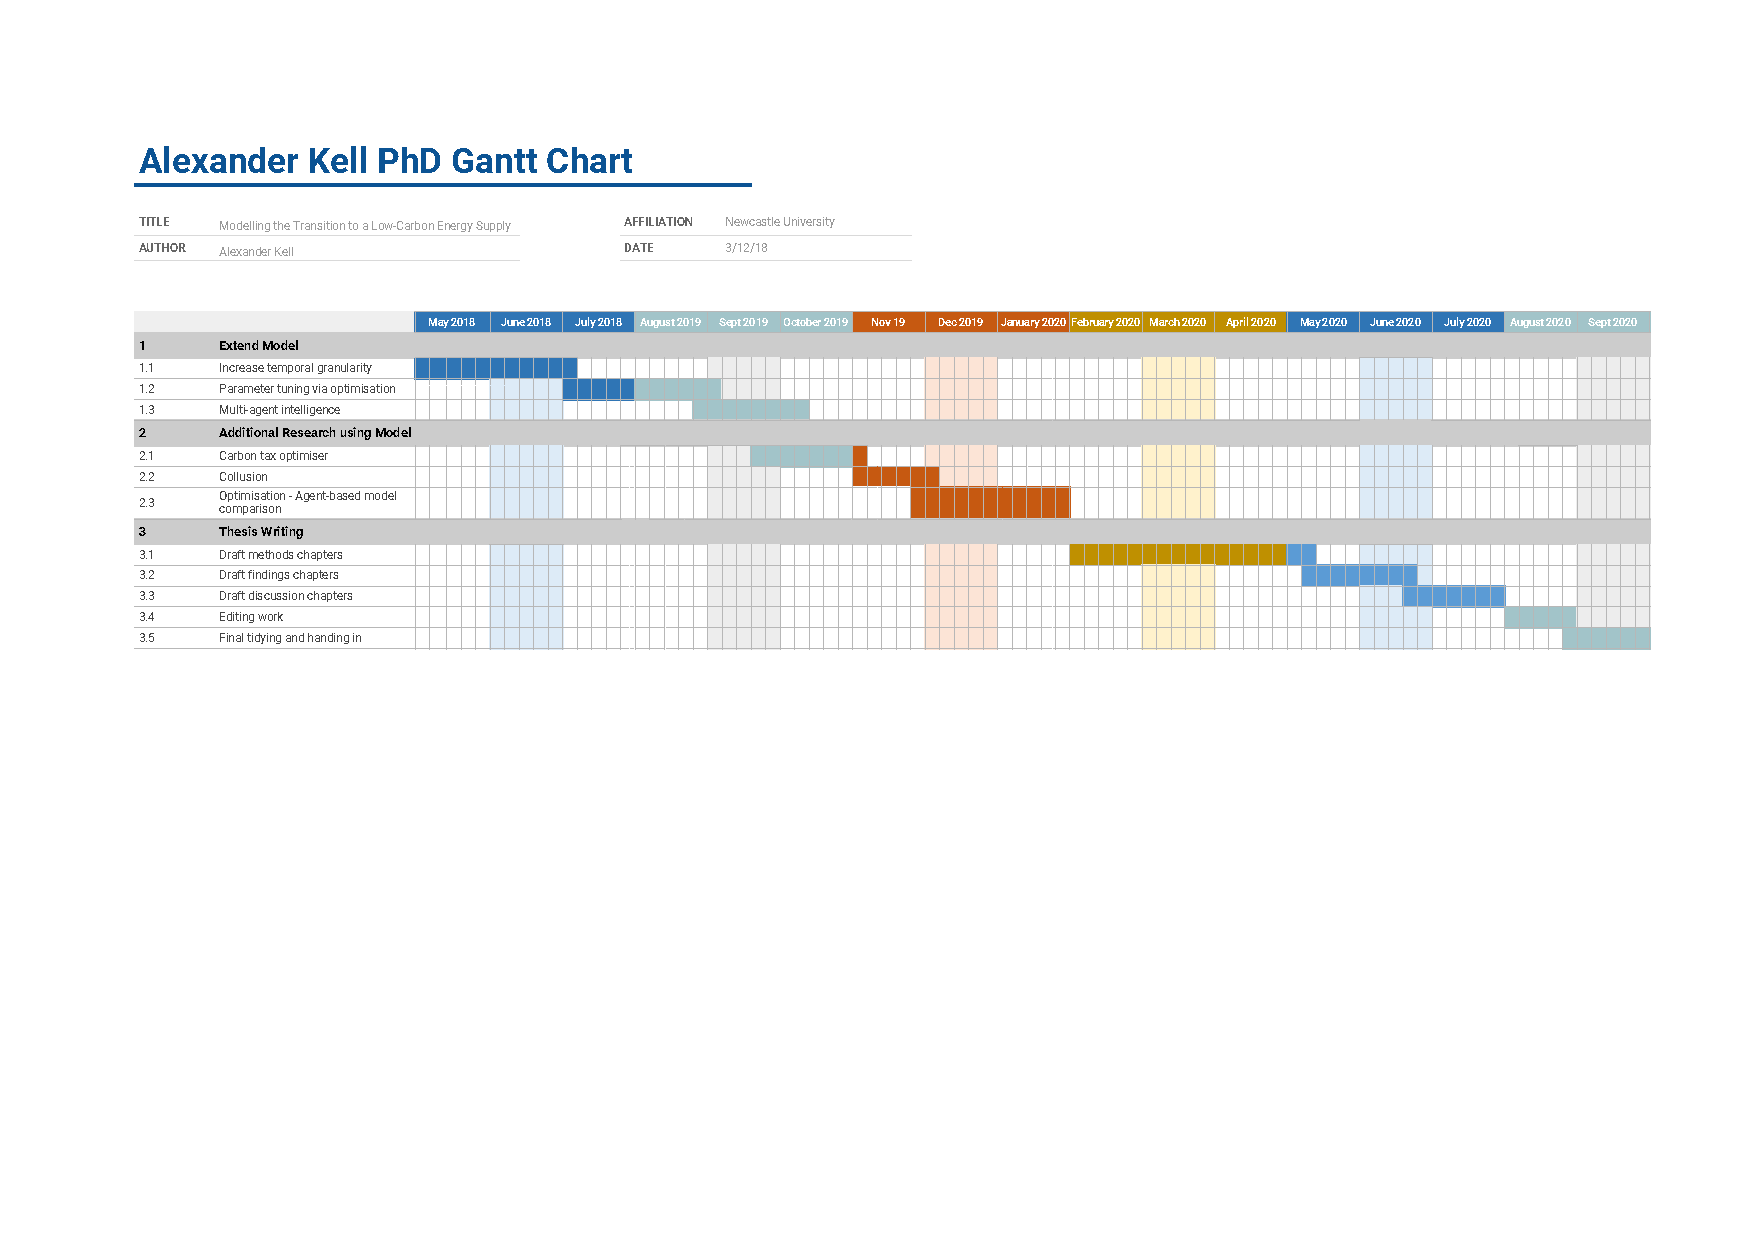
\includepdf[landscape=true]{gantt.pdf}








\clearpage

\section{Thesis Outline}

\subsection{Chapters}
\begin{enumerate}

  \item Introduction
  \item Literature review
  \item Data analytics of smart meter data
  \begin{enumerate}
	  \item Short-term 
	  \item Long-term load forecasting (inadequacy of long-term load forecasting)
	  \item Demand segmentation
  \end{enumerate}
  \item ElecSim: An open-sourced agent-based model
    \begin{enumerate}
	  \item Yearly granularity
	  \item Hourly granularity
  \end{enumerate}
  \item Adding Intelligence to Agents
  \begin{enumerate}
	  \item Reinforcement learning techniques for agents
	  \item Collusion
	  \item Optimisation of Carbon Tax using reinforcement learning
  \end{enumerate}
  \item Scenarios
  \item Agent-based model and Optimisation tool: A comparison
  \item Conclusion and future work
  
\end{enumerate}












\clearpage

\bibliography{library,custom}
\bibliographystyle{ieeetr}
\end{document}
